\documentclass[12pt]{article}
\usepackage[utf8]{inputenc}
\usepackage{geometry}
\usepackage{amsfonts}
\usepackage{hyperref}
\usepackage{enumitem}
\usepackage{graphicx}
\usepackage{tabularx}
\usepackage{amsmath}
\usepackage{xcolor}


\title{
    \textbf{CSE343: Machine Learning} \\ \vspace*{-5pt}
    \textbf{\large{Assignment-1}}
}

\author{\href{mailto:divyajeet21529@iiitd.ac.in}{Divyajeet Singh (2021529)}}
\date{\today}

\geometry{a4paper, left=20mm, right=20mm, top=20mm, bottom=20mm}


\begin{document}
    \maketitle

    \section{Section A (Theoretical)}

    \subsubsection*{(a) (2 marks)}
    If two variables exhibit a strong correlation with a third variable, does this necessarily imply that they will also display
    a high degree of correlation with each other? Provide a reasoned explanation, supported by an illustrative example.

    \subsubsection*{Solution}
    No. When two variables exhibit a strong correlation with a third variable, they may or may not display a high degree of
    correlation with each other. This is because the correlation between two variables is a measure of the linear relationship
    between them. It does not imply that the two variables are dependent on each other.
    \vspace*{5pt} \\
    As an example, consider two independent variables $X_{1}$ and $X_{2}$. Consider a variable $W$, which is a linear combination
    of $X_{1}$ and $X_{2}$, let's say
    \begin{equation}
        W = X_{1} + X_{2}
    \end{equation}
    Then, $X_{1}$ and $W$ are
    strongly correlated, and $X_{2}$ and $W$ are also strongly correlated. However, $X_{1}$ and $X_{2}$ are not correlated at all.

    \subsubsection*{(b) (2 marks)}
    What is the defining criteria(s) for a mathematical function to be categorized as a logistic function? Briefly explain which
    of the following functions are valid logistic functions: $\sinh{(x)}$, $\cosh{(x)}$, $\tanh{(x)}$, and $\text{signum}{(x)}$.

    \subsubsection*{Solution}
    Mathematically, a function $f: \mathbb{R} \to \mathbb{R}$ is a logistic function if it is bounded, continuous, and can be written
    in the form \begin{equation}
        \label{eq:logistic}
        f(x) = \frac{A}{1 + e^{-B(x - x_{0})}} + C
    \end{equation}
    where the parameters are
    \begin{itemize}[noitemsep]
        \item $A \in \mathbb{R}$: the curve's maximum asymptote when $C = 0$
        \item $B \in \mathbb{R}^{+}$: the logistic growth rate or steepness of the curve
        \item $x_{0} \in \mathbb{R}$: the $x$-value of the sigmoid's midpoint
        \item $C \in \mathbb{R}$: a scalar to shift the curve vertically
    \end{itemize}
    This means that the function must be limited within its two horizontal asymptotes.
    Given the above constraints, the hyperbolic functions $\sinh{(x)}$ and $\cosh{(x)}$ are not valid logistic functions,
    simply because they are unbounded over $\mathbb{R}$.
    \begin{align*}
        \lim_{x \to \pm \infty} \sinh{(x)} &= \lim_{x \to \pm \infty} \frac{e^{x} - e^{-x}}{2} \to \pm \infty \\
        \lim_{x \to \pm \infty} \cosh{(x)} &= \lim_{x \to \pm \infty} \frac{e^{x} + e^{-x}}{2} \to +\infty \\
    \end{align*}
    The function $\tanh{(x)}$ can be written in the form of \eqref{eq:logistic} with the assignment $A = 2$, $B = 2$,
    $x_{0} = 0$, and $C = -1$.  Moreover, $\tanh{(x)}$ is continuous and bounded over $\mathbb{R}$.
    Hence, it is a valid logistic function. A simple derivation is given below.
    \begin{align*}
        \tanh{(x)} &= \frac{\sinh{(x)}}{\cosh{(x)}} = \frac{e^{x} - e^{-x}}{e^{x} + e^{-x}} \\
        &= \frac{1 - e^{-2x}}{1 + e^{-2x}} = \frac{2}{1 + e^{-2x}} - \frac{1 + e^{-2x}}{1 + e^{-2x}} \\
        &= \frac{2}{1 + e^{-2x}} - 1
    \end{align*}
    \vspace*{5pt} \\
    The function $\text{signum}{(x)}$ is not a valid logistic function, because it is not continuous over $\mathbb{R}$.

    \begin{figure}[h]
        \centering
        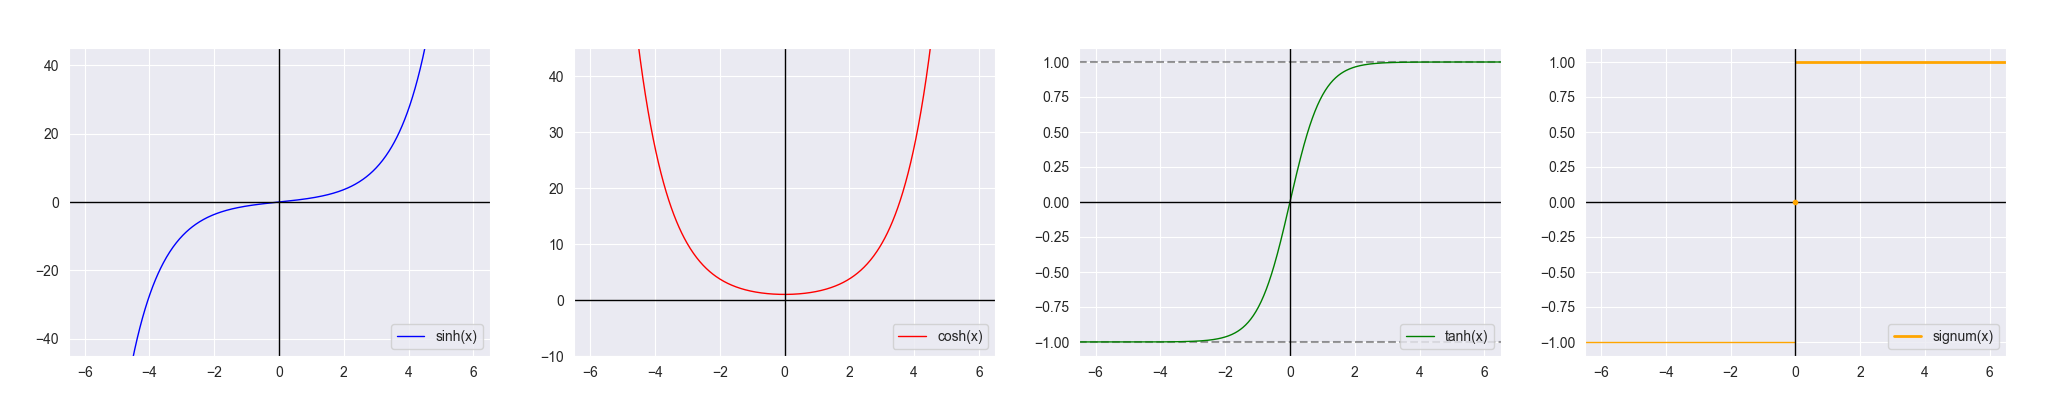
\includegraphics[width=1.0\textwidth]{./../Assets/plots.png}
        \caption{Plots of $\sinh{(x)}$, $\cosh{(x)}$, $\tanh{(x)}$, and $\text{signum}{(x)}$}
    \end{figure}

    \subsubsection*{(c) (2 marks)}
    Which validation technique is beneficial for very sparse datasets and why? Briefly explain how it is different from the
    traditional $k$-fold cross-validation technique.

    \subsubsection*{Solution}
    Leave-one-out Cross-Validation (LooCV) is beneficial for sparse datasets. On a dataset with $N$ samples, LooCV trains a model
    on $N - 1$ samples and tests it on the remaining sample. This is repeated $N$ times, selecting a different sample for testing
    each time. This way, $N$ different models are trained and tested, and the average error is reported.
    \vspace*{5pt} \\
    For sparse datasets with small number of samples, this is beneficial because it ensures that the models are trained on as
    large of a subset of the data as possible, which should ideally decrease both bias and variance.
    \vspace*{5pt} \\
    Comparitively, in the $k$-fold Cross Validation technique, the dataset is divided into $k$ folds of size $\frac{N}{k}$
    each. $k$ models are trained on $k$ different subsets of size $\frac{N}{k} \cdot (k - 1)$ and tested on the remaining fold,
    where $k \leq N$ and $k \in \mathbb{N}$. With $k = N$, this technique is equivalent to LooCV.

    \subsubsection*{(d) (2 marks)}
    Find the coefficients of the least square regression line for a set of $n$ data points $(x_{i}, y_{i})$ in slope-intercept form.

    \subsubsection*{Solution}
    The Least Square Regression technique of linear regression assumes that the label for each data point is a linear combination
    of the features. In other words, the label $y_{i} \ (0 \leq i \leq n)$ for a data point $(x_{i}, y_{i})$ is given by
    \begin{equation}
        y_{i} = b_{0} + b_{1} x_{i} + \epsilon_{i}
    \end{equation}
    where $\epsilon_{i}$ is the error, assumed to be randomly drawn from an unknown normal distribution $\epsilon \sim N[0, \sigma^{2}]$.
    Hence, the problem is to find parameters $b_{0}$ and $b_{1}$ that give the line that best fits the data.
    \vspace*{5pt} \\
    Given $n$ data points, this is an optimization problem to minimize the mean residual sum of squares.
    \begin{align}
        \min_{\mathbf{b}} J(\mathbf{b} := (b_{0}, b_{1})) &= \min_{\mathbf{b}} \frac{1}{n} \sum_{i=1}^{n} \epsilon_{i}^{2} \\
        &= \min_{\mathbf{b}} \frac{1}{n} \sum_{i=1}^{n} (y_{i} - b_{0} - b_{1} x_{i})^{2}
    \end{align}
    This can be solved by finding the gradient of $J(\mathbf{b})$ and setting it to $0$.
    \begin{align}
        \frac{\partial J(\mathbf{b})}{\partial b_{0}} = 0
        &\implies \frac{2}{n} \sum_{i=1}^{n} (y_{i} - b_{0} - b_{1} x_{i}) \cdot (-1) = 0 \\
        &\implies \frac{1}{n} \sum_{i=1}^{n} (b_{0} + b_{1} x_{i} - y_{i}) = 0 \\
        &\implies b_{0} + b_{1} \cdot \frac{1}{n} \sum_{i=1}^{n} x_{i} - \frac{1}{n} \sum_{i=1}^{n} y_{i} = 0 \\
        &\implies b_{0} = \frac{1}{n} \sum_{i=1}^{n} y_{i} - b_{1} \left( \frac{1}{n} \sum_{i=1}^{n} x_{i} \right) \\
        &\implies b_{0} = \bar{y} - b_{1} \bar{x}
        \\[15pt]
        \frac{\partial J(\mathbf{b})}{\partial b_{1}} = 0
        &\implies \frac{2}{n} \sum_{i=1}^{n} (y_{i} - b_{0} - b_{1} x_{i}) \cdot (-x_{i}) = 0 \\
        &\implies b_{1} \sum_{i=1}^{n} x_{i}^{2} + b_{0} \sum_{i=1}^{n} x_{i} - \sum_{i=1}^{n} x_{i} y_{i} = 0 \\
        &\implies b_{1} \sum_{i=1}^{n} x_{i}^{2} + (\bar{y} - b_{1} \bar{x}) \cdot n \bar{x} = \sum_{i=1}^{n} x_{i} y_{i} \\
        &\implies b_{1} \left( \sum_{i=1}^{n} x_{i}^{2} - n \bar{x}^{2} \right) = \sum_{i=1}^{n} x_{i} y_{i} - n \bar{x} \bar{y} \\
        &\implies b_{1} = \frac{\sum_{i=1}^{n} x_{i} y_{i} - n \bar{x} \bar{y}}{\sum_{i=1}^{n} x_{i}^{2} - n \bar{x}^{2}}
    \end{align}
    \vspace*{5pt} \\
    So, the line $Y = b_{0} + b_{1} X$ is the line of best fit for the given data points, where $b_{0}$ and $b_{1}$ are given
    by the above equations.

    \subsubsection*{(e) (1 mark)}
    What parameters are to be estimated in the simple linear regression model $Y = \alpha + \beta x + \epsilon$, where
    $\epsilon \sim N[0, \sigma^{2}]$?

    \subsubsection*{Solution}
    In a simple linear model of regression, the parameters to be estimated are $\alpha$, $\beta$, and $\sigma$. The parameter
    $\beta$ is the slope of the regression line, $\alpha$ is its intercept, and $\sigma$ is the standard
    deviation of the error term $\epsilon$.
    \vspace*{5pt} \\
    The parameters $\alpha$ and $\beta$ are estimated using the least squares method. The parameter $\sigma^{2}$ is estimated as
    the variance of the residuals/errors, i.e. the difference between the observed and estimated values of $Y$.
    \begin{equation}
        \sigma^{2} = \frac{1}{n-2} \sum_{i=1}^{n} (y_{i} - \hat{y}_{i})^{2} \implies
        \sigma = \sqrt{\frac{\sum_{i=1}^{n} (y_{i} - \hat{y}_{i})^{2}}{n - 2}}
    \end{equation}
    where we divide by $n - 2$ instead of $n$ because we have estimated two parameters, which means two degrees of freedom are lost.
    \vspace*{5pt} \\
    The error term $\epsilon$ is assumed to be a fixed random number drawn from a normal distribution with mean $0$ and
    variance $\sigma^{2}$. Hence, there is no need to estimate the error.

    \subsubsection*{(f) (1 mark)}
    In a study of the relationship between the mean daily temperature for the month and monthly charges on the electric bill,
    the following data was gathered:
    \begin{align*}
        X = \text{mean daily temperature} &= [ 20, 30, 50, 60, 80, 90 ] \\
        Y = \text{monthly electric bill charges} &= [ 125, 110, 95, 90, 110, 130 ]
    \end{align*}
    Which of the following seems the most likely model?
    \begin{enumerate}[label=(\alph*), noitemsep]
        \item $Y = \alpha + \beta x + \epsilon \quad \beta < 0$
        \item $Y = \alpha + \beta x + \epsilon \quad \beta > 0$
        \item $Y = \alpha + \beta_{1} x + \beta_{2} x^{2} + \epsilon \quad \beta_{2} < 0$
        \item $Y = \alpha + \beta_{1} x + \beta_{2} x^{2} + \epsilon \quad \beta_{2} > 0$
    \end{enumerate}

    \subsubsection*{Solution}
    Given $X$ and $Y$, it is easy to notice that as the mean daily temperature increases, the monthly electric bill charges
    first decrease and then increase again.
    Hence, it is likely that the relationship between $X$ and $Y$ is quadratic.
    \vspace*{5pt} \\
    Let the model be $Y = \alpha + \beta_{1} x + \beta_{2} x^{2} + \epsilon$. Then, we can observe the following
    \begin{align}
        Y &= \alpha + \beta_{1} x + \beta_{2} x^{2} + \epsilon \\
        \implies \frac{dY}{dx} &= \beta_{1} + 2 \beta_{2} x \\
        \label{eq:derivative}
        \implies \frac{d^{2}Y}{dx^{2}} &= 2 \beta_{2} > 0 \implies \beta_{2} > 0
    \end{align}
    The drop and rise in $Y$ values with increase in $x$ values means that the first derivative of $Y$ with respect to $x$
    increases from negative to positive, indicating that the second derivative is positive. This relationship is
    highlighted in \eqref{eq:derivative}.
    \vspace*{5pt} \\
    The model cannot be linear, since the second derivative of a linear model will be $0$ for all values of $x \in \mathbb{R}$.
    Hence, the most likely model is (d).

    \section{Section B (Scratch Implementation)}

    This problem is about implementing the Logistic Regression algorithm with Stochastic Gradient Descent from scratch.
    The \href{https://drive.google.com/file/d/1p7ivBMLoT-Zxp8_9Pt8n8oWUjqLdBxPN/view?usp=drive_link}{
        \textbf{\color{blue}{Diabetes Healthcare Dataset}}
    } was used for this problem. The implementation can be found in \texttt{utils.py}.

    \subsection*{Convergence of the Model}
    We start with a base model with $\alpha = 0.005$ and 70 epochs. This model gives a fairly consistent performance
    and convergess to a loss of less than $0.5$ within less than 70 epochs. The loss and accuracy plots for this model are shown in
    Figure \ref{fig:base_model}.
    \vspace*{5pt} \\
    This model also displays low bias and low variance, with an average accuracy of about $75\%+$.
    \begin{figure}[h]
        \centering
        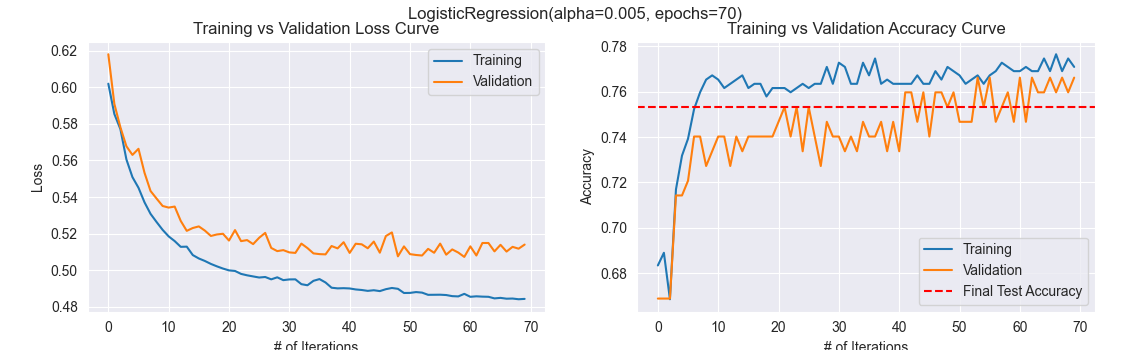
\includegraphics[width=0.85\textwidth]{./../Assets/base_model.png}
        \caption{Loss and Accuracy plots for the base model}
        \label{fig:base_model}
    \end{figure}

    \subsection*{Hyperparameter Testing - Models with different Learning Rates}
    Different models were trained with different values of the learning rate. The results of the models are compared in the
    following figures.
    \begin{figure}[h]
        \centering
        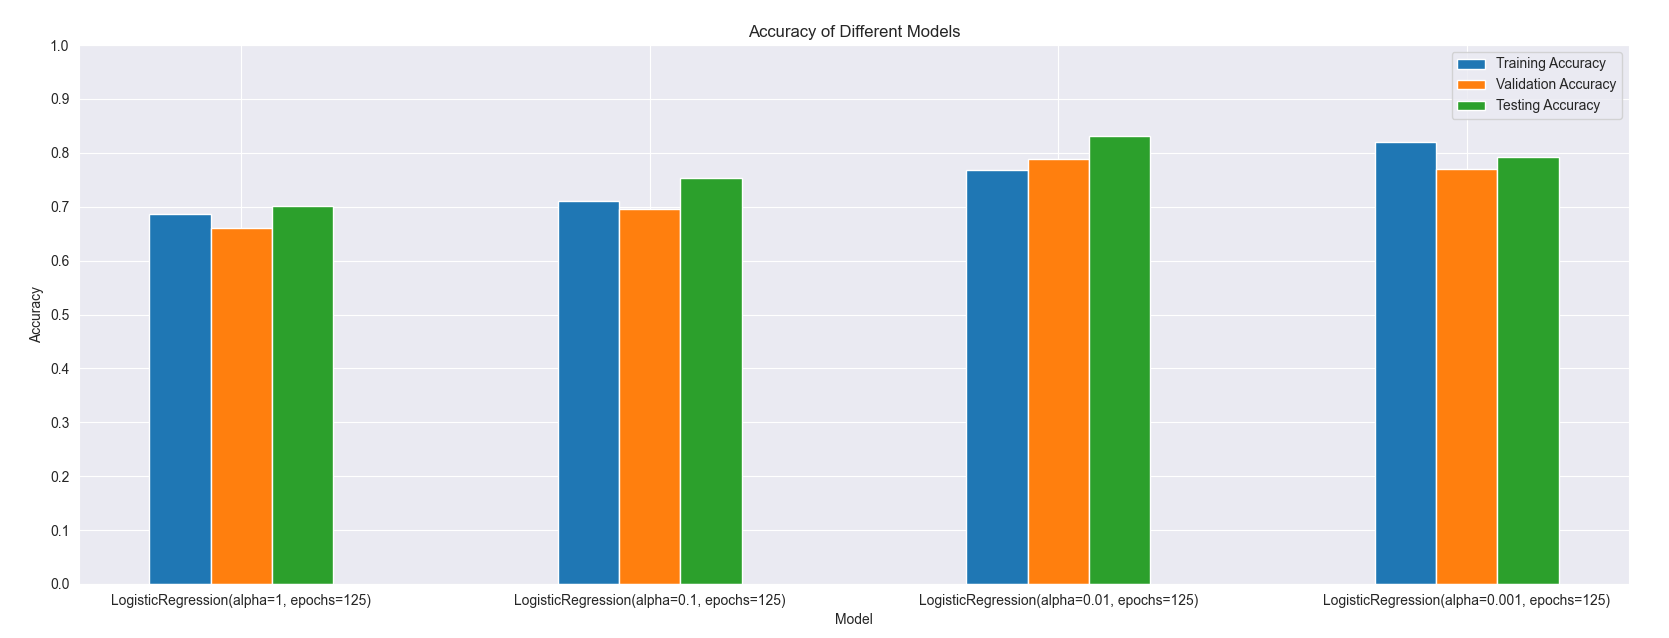
\includegraphics[width=0.85\textwidth]{./../Assets/accuracy.png}
        \caption{Training, Testing, and Validation Accuracy for different learning rates}
        \label{fig:accuracy}
    \end{figure}
    \vspace*{5pt} \\
    Figure \ref{fig:accuracy} suggests that learning rates $1.0$ and $0.1$ are too high, and so the model does not converge
    to a good estimate of the weights. With sufficient number of epochs the models with $\alpha = 0.01$ and $\alpha = 0.001$
    perform well. However, the model with $\alpha = 0.001$ converges slower than the model with $\alpha = 0.01$ and
    hence takes more epochs to train.
    \begin{figure}[h]
        \centering
        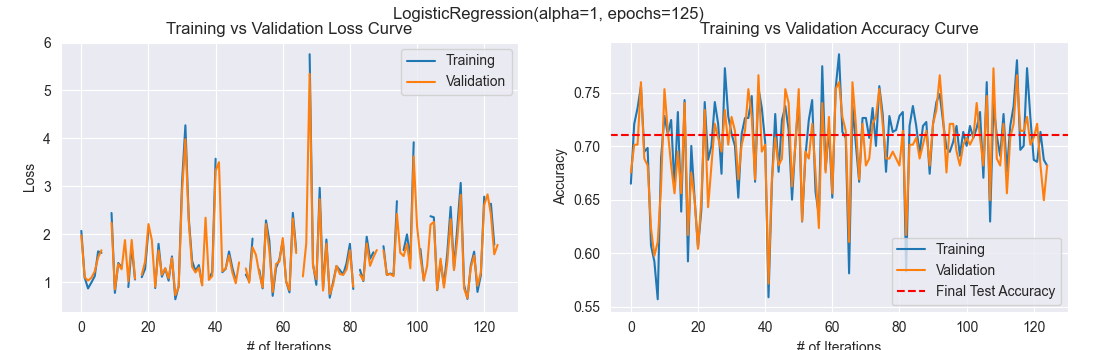
\includegraphics[width=0.85\textwidth]{./../Assets/model_1.png}
        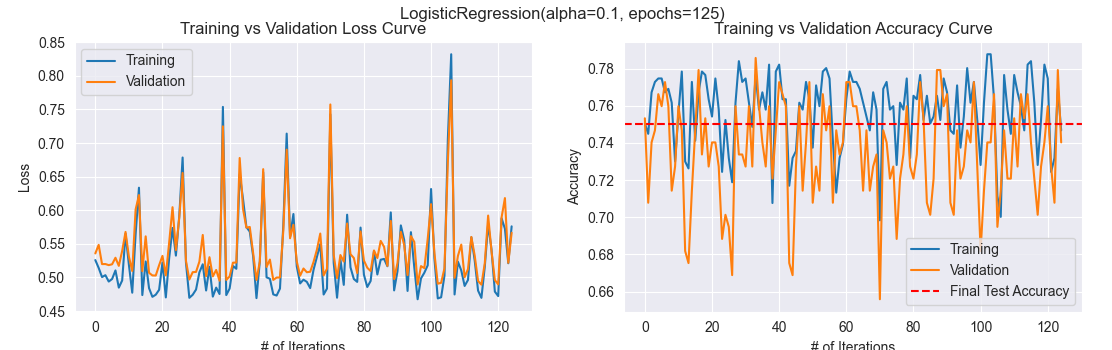
\includegraphics[width=0.85\textwidth]{./../Assets/model_2.png}
        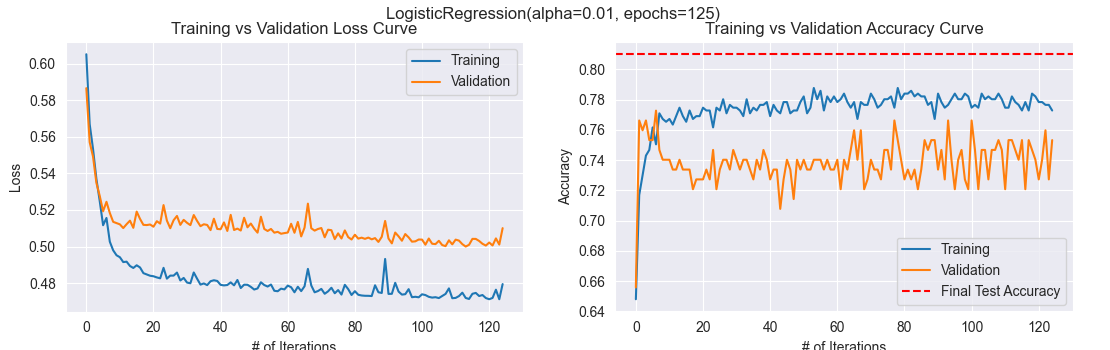
\includegraphics[width=0.85\textwidth]{./../Assets/model_3.png}
        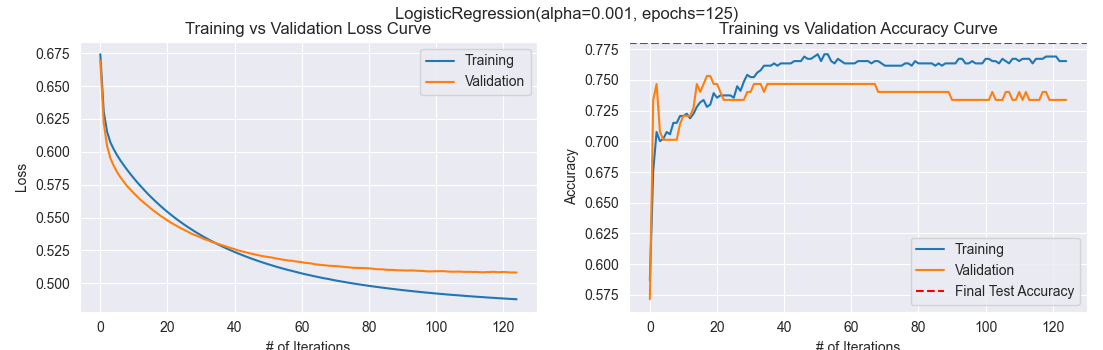
\includegraphics[width=0.85\textwidth]{./../Assets/model_4.png}
        \caption{Loss and Accuracy plots for models with different learning rates}
        \label{fig:models}
    \end{figure}
    \vspace*{5pt} \\
    Figure \ref{fig:models} clearly demonstrates the difference in convergence between the models.
    The model with $\alpha = 0.001$ converges more smoothly, and with more than 50 epochs, it sometimes performs better
    than the other models.
    \vspace*{5pt} \\
    We also look at the confusion matrices of the four models to see how they perform on the test set.
    The confusion matrix is structured as follows.
    \begin{equation}
        CM = \begin{bmatrix}
            TP & FP \\
            FN & TN
        \end{bmatrix}
    \end{equation}
    \begin{figure}[h]
        \centering
        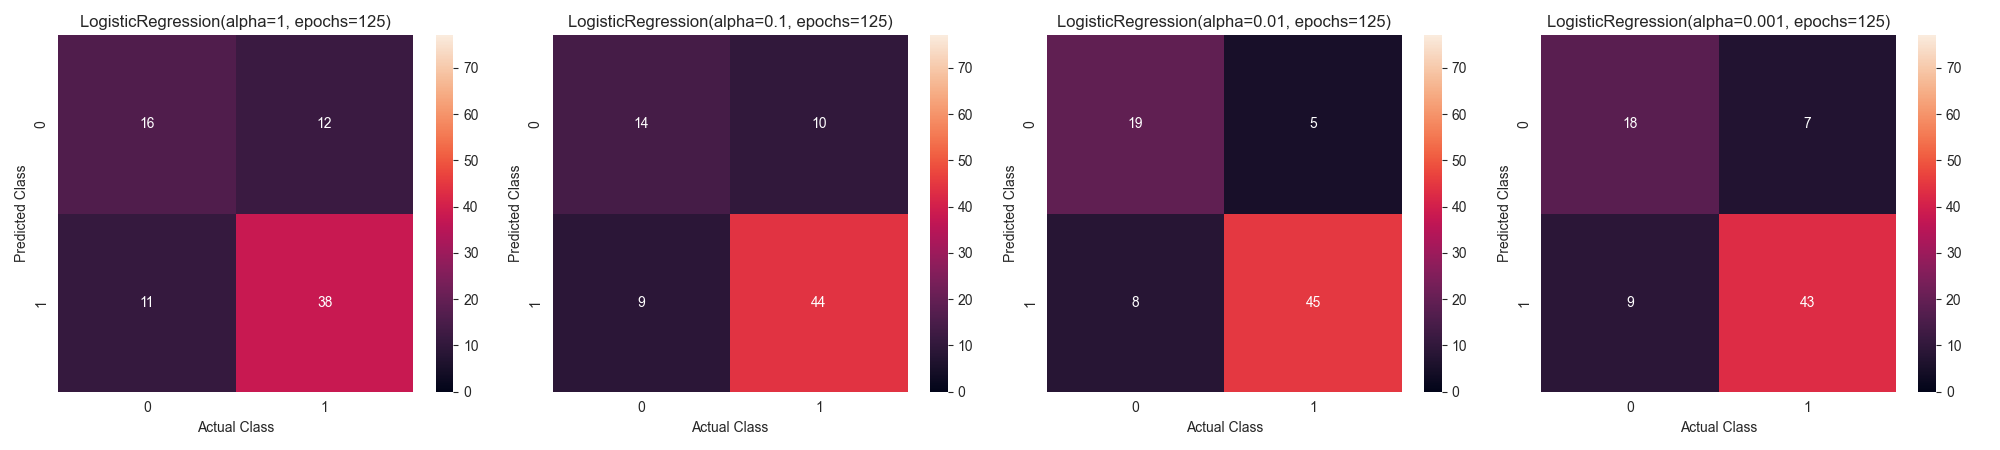
\includegraphics[width=0.9\textwidth]{./../Assets/confusion_matrices.png}
        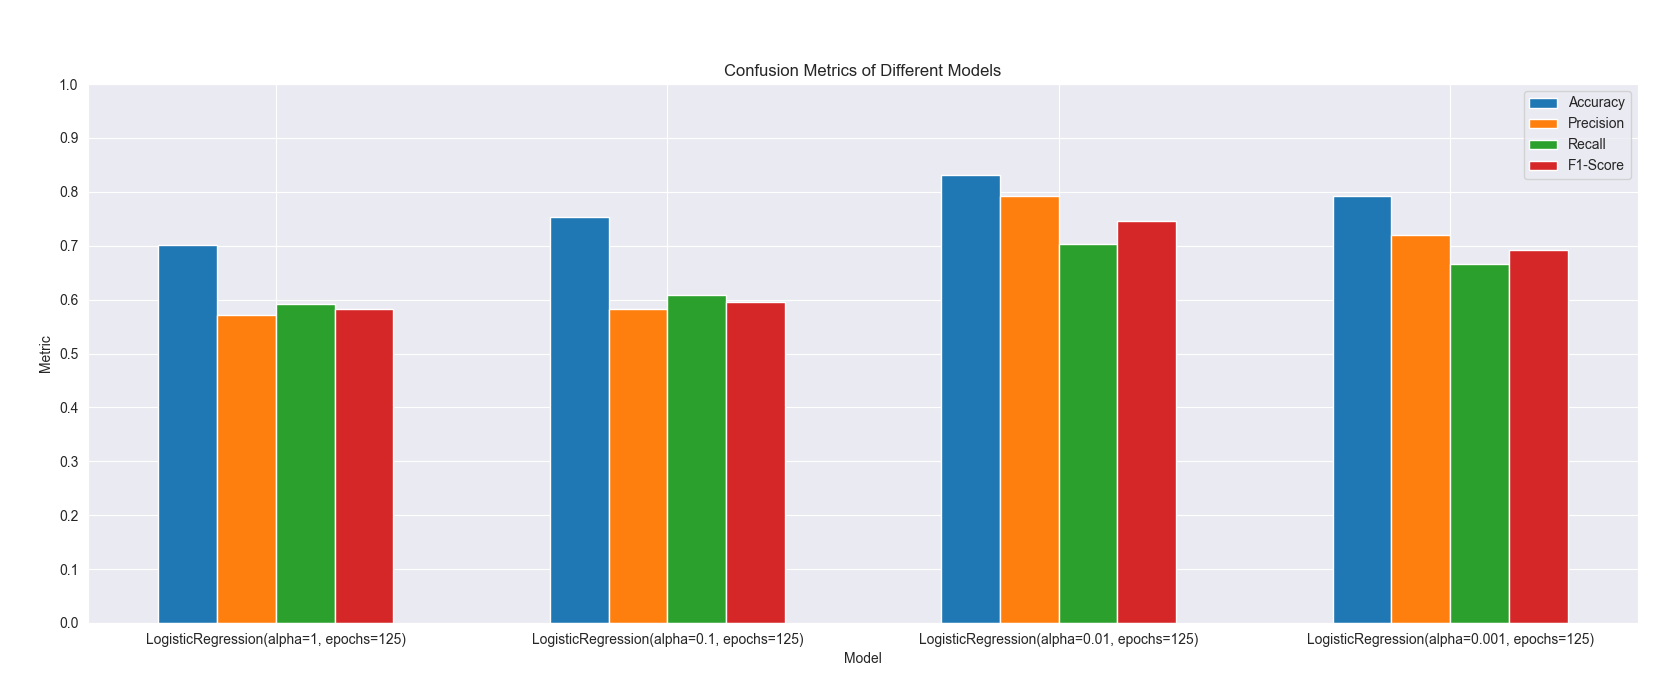
\includegraphics[width=0.9\textwidth]{./../Assets/confusion_metrics.png}
        \caption{Confusion matrices and metrics for models with different learning rates}
        \label{fig:confusion}
    \end{figure}
    \vspace*{0pt} \\
    Figure \ref{fig:confusion} shows a comparison between the confusion matrices and metrics - Accuracy, Precision, Recall, and
    F1-Score of the four models. The model with $\alpha = 0.01$ performs the best, with the highest
    true results and least false results, and best metrics.

    \subsection*{Adding Regularization to the Models}
    We now add regularization to the models to see if it improves the performance. The regularization terms $L_{1}$ and $L_{2}$
    are added to the cross-entropy loss $J(\theta)$ to get the regularized loss functions
    $J_{L_{1}}(\theta)$ and $J_{L_{2}}(\theta)$.
    \begin{align}
        L_{1} &= \lambda \sum_{j=1}^{d} |\theta_{j}| \\
        L_{2} &= \lambda \sum_{j=1}^{d} \theta_{j}^{2} \\
        J_{L_{k}}(\theta) &= J(\theta) + L_{k}
    \end{align}
    We search over a range of values of $\lambda$ to find the best value for both regularization terms. The training and
    validation loss and accuracy per iteration is given in Figure \ref{fig:regularization}.
    \begin{figure}[h]
        \centering
        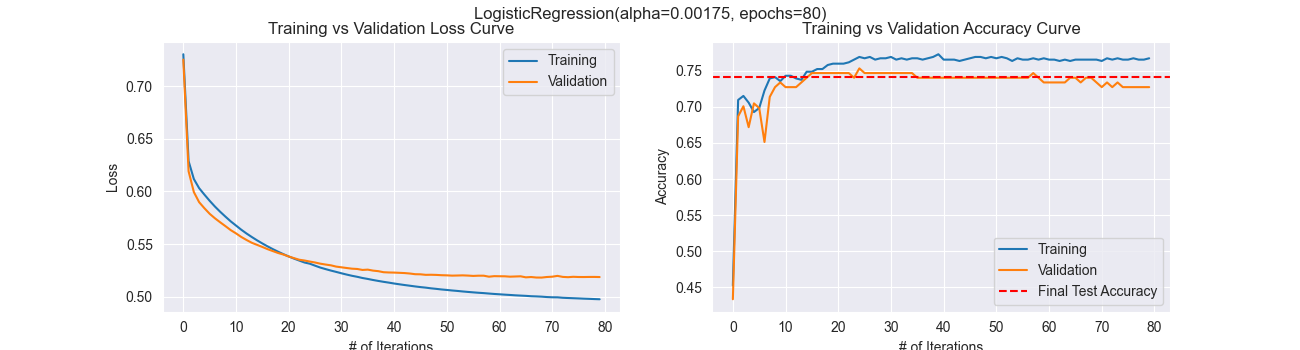
\includegraphics[width=0.9\textwidth]{./../Assets/reg_l1.png}
        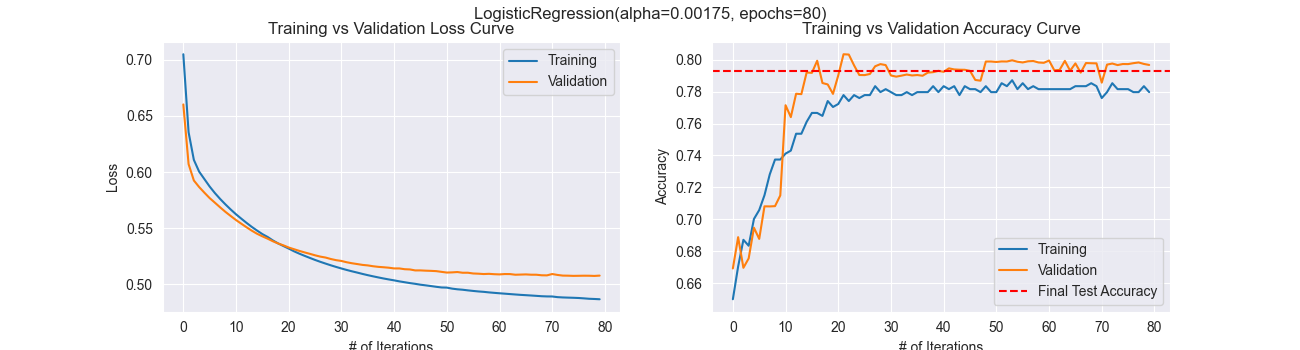
\includegraphics[width=0.9\textwidth]{./../Assets/reg_l2.png}
        \caption{Training and Validation Loss and Accuracy for $L_{1}$ and $L_{2}$ regularization}
        \label{fig:regularization}
    \end{figure}
    \vspace*{5pt} \\
    Regularization tends to make the performance of the models more consistent. With any sufficient learning rate, adding
    regularization to the loss and gradient helped decrease the variance in the performance on training and validation sets.
    \vspace*{5pt} \\
    For $L_{1}$ regularization, the best value of $\lambda$ was in $[0.001, 0.0001]$. For $L_{2}$ regularization,
    the best value of $\lambda$ was around $10^{-4}$.

    \subsection*{Changing the logistic function to $\tanh{(x)}$}
    We now change the logistic function from the sigmoid function to the hyperbolic tangent function $\tanh{(x)}$.
    The range of $\tanh{(x)}$ is $[-1, 1]$, so it was normalized to $[0, 1]$ by adding $1$ and dividing by $2$.
    Our new hypothesis function becomes
    \begin{equation}
        h_{\theta}(x) = \frac{1}{2} \cdot (1 + \tanh{(\theta^{T} x)})
    \end{equation}
    We still choose to use the Bianry Cross-Entropy loss function, since it is a good measure of the performance of the model.
    However, the gradient was changed according to the new hypothesis function.
    \vspace*{5pt} \\
    The training and validation loss and accuracy per iteration is given in Figure \ref{fig:tanh}.
    \begin{figure}[h]
        \centering
        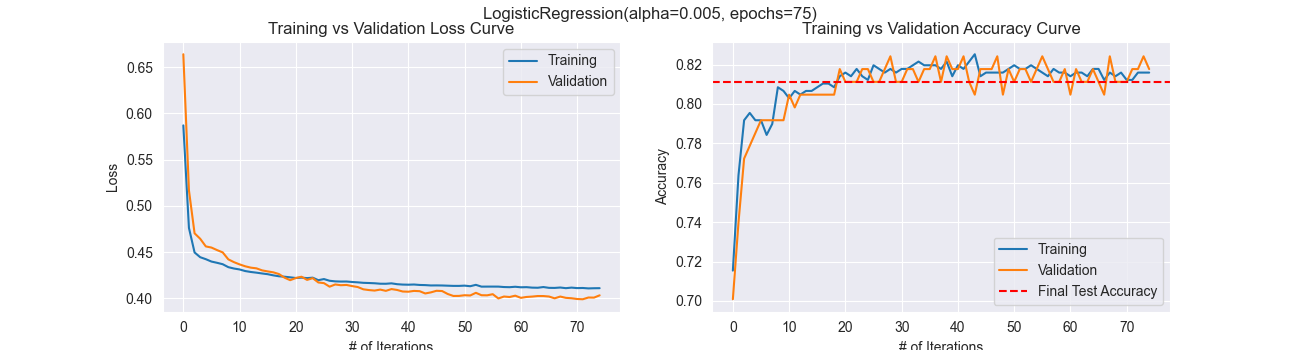
\includegraphics[width=0.9\textwidth]{./../Assets/tanh.png}
        \caption{Training and Validation Loss and Accuracy for $\tanh{(x)}$}
        \label{fig:tanh}
    \end{figure}
    On average, the model using $\tanh{(x)}$ performed better than the model using the sigmoid function. Using $\tanh{(x)}$
    also makes the model converge in a lot less epochs, and the model converges to a better loss value. This could be
    attributed to the difference in gradients of the two functions.

    \subsection*{Implementing Mini-Batch Gradient Descent}
    Finally, the model was trained using Mini-Batch Gradient Descent, with different values for the batch-size parameter.
    It was observed that as batch-size increases, the model converges faster. With batch-size, the model performance
    also increases, however, it stabilizes when batch-size is close to half the size of the training set.
    \vspace*{5pt} \\
    The average performance is also better than model using SGD. This is because in each epoch, the model gets exposed to more
    training data, and hence, learns better.
    \begin{figure}[h]
        \centering
        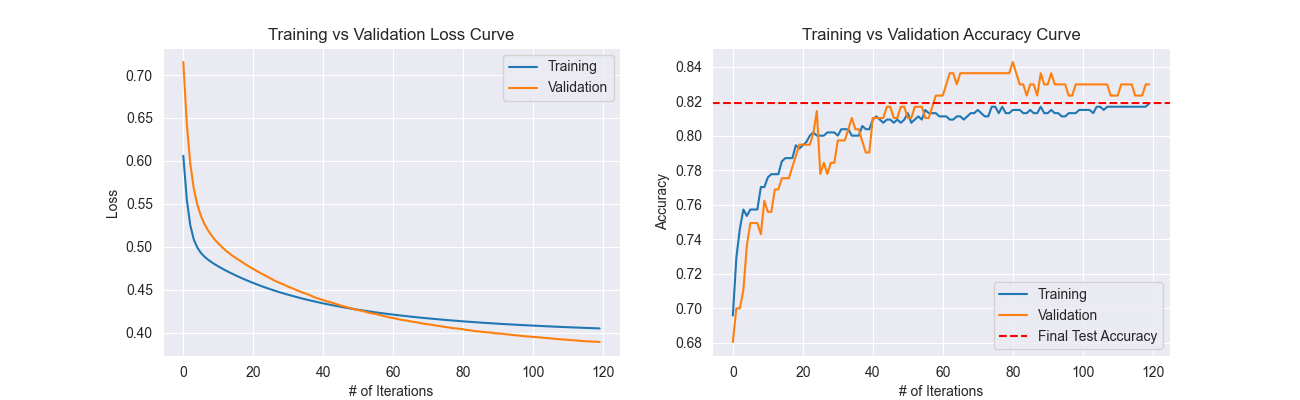
\includegraphics[width=0.9\textwidth]{./../Assets/mini_bgd.png}
        \caption{Training and Validation Loss and Accuracy for Mini-Batch Gradient Descent}
        \label{fig:mini_batch}
    \end{figure}
    \vspace*{0pt} \\
    Figure \ref{fig:mini_batch} shows the training and validation loss and accuracy per iteration for an instance of Mini-BGD,
    at batch-size $= 275$. It is hence, easy to note that Mini-BGD models converge a little faster than SGD models.

    \section{Section C (Algorithm Implementation using Packages)}

    This problem is about implementing the Linear Regression algorithm using the \texttt{scikit-learn} package.
    The \href{https://drive.google.com/file/d/1Ei_-dA3MOafI5cWPP_l4dfUAkofzesyM/view?usp=sharing}{
        \textbf{\color{blue}{CO$_{2}$ Emissions Dataset}}
    } was used for this problem. The data analysis and model training can be fiund in the main notebook.

    \subsection*{Data Analysis}
    The data was analyzed to find relevant features, and the features that are correlated to the target variable,
    \texttt{CO2 Emissions (g/km)}. The distributions of the features were also plotted to see if they are normally
    distributed. \\
    \begin{figure}[h]
        \centering
        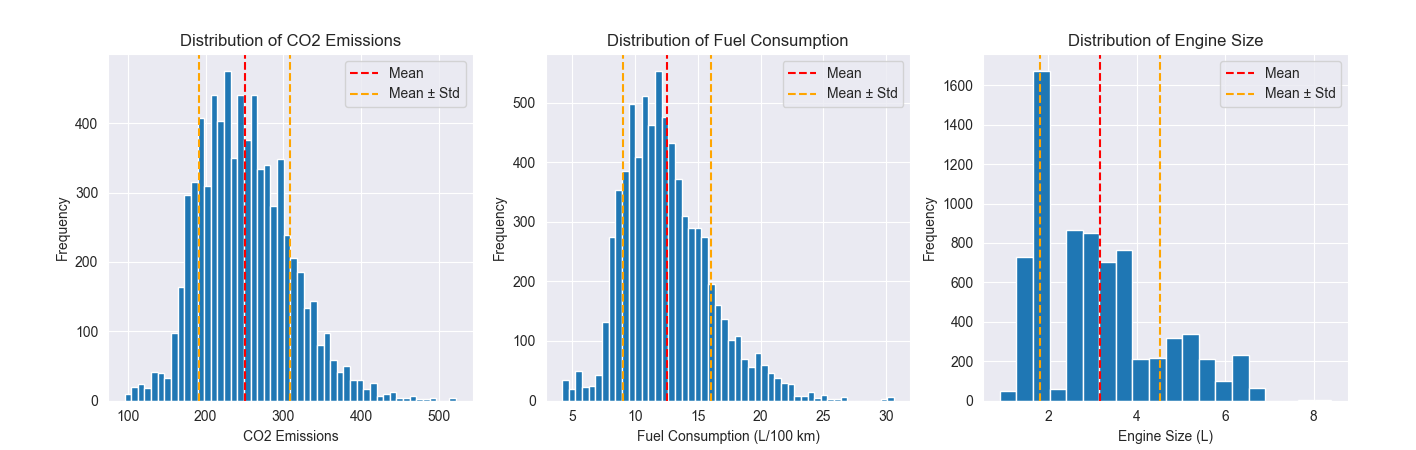
\includegraphics[width=0.95\textwidth]{./../Assets/distribution.png}
        \caption{Distribution of some variables}
        \label{fig:distribution}
    \end{figure}
    \vspace*{5pt} \\
    Figure \ref{fig:distribution} shows the distribution of the target variable, and features like \texttt{Engine Size(L)}
    and \texttt{Fuel Consumption Comb (L/100 km)}. The distribution of each of them is almost gaussian, with a slight
    skew towards the left.
    \vspace*{5pt} \\
    Figure \ref{fig:pairplot} shows the pairplot of the features against each other. It is easy to note that most
    features show a strong positive correlation with each other. The feature \texttt{Fuel Consumption Comb (mpg)} shows
    a strong negative correlation with the other features. Moreover, the target variable also shows a storng correlation
    with all features. The correlation matrix of the data is given in Figure \ref{fig:correlation}.
    \vspace*{5pt} \\
    Figure \ref{fig:box} shows the boxplot of the feature \texttt{Vehicle Class}. It is easy to note that the median
    \texttt{CO2 Emissions} for \texttt{Vehicle Class} \texttt{VAN - PASSENGER} is the highest, and the median \texttt{CO2 Emissions}
    for \texttt{Vehicle Class} \texttt{STATION WAGON - SMALL} is the lowest. Moreover, the \texttt{Vehicle Class} of
    \texttt{COMPACT} and \texttt{MID-SIZE} have the largest variance (and hence number of outliers).
    \begin{figure}[h]
        \centering
        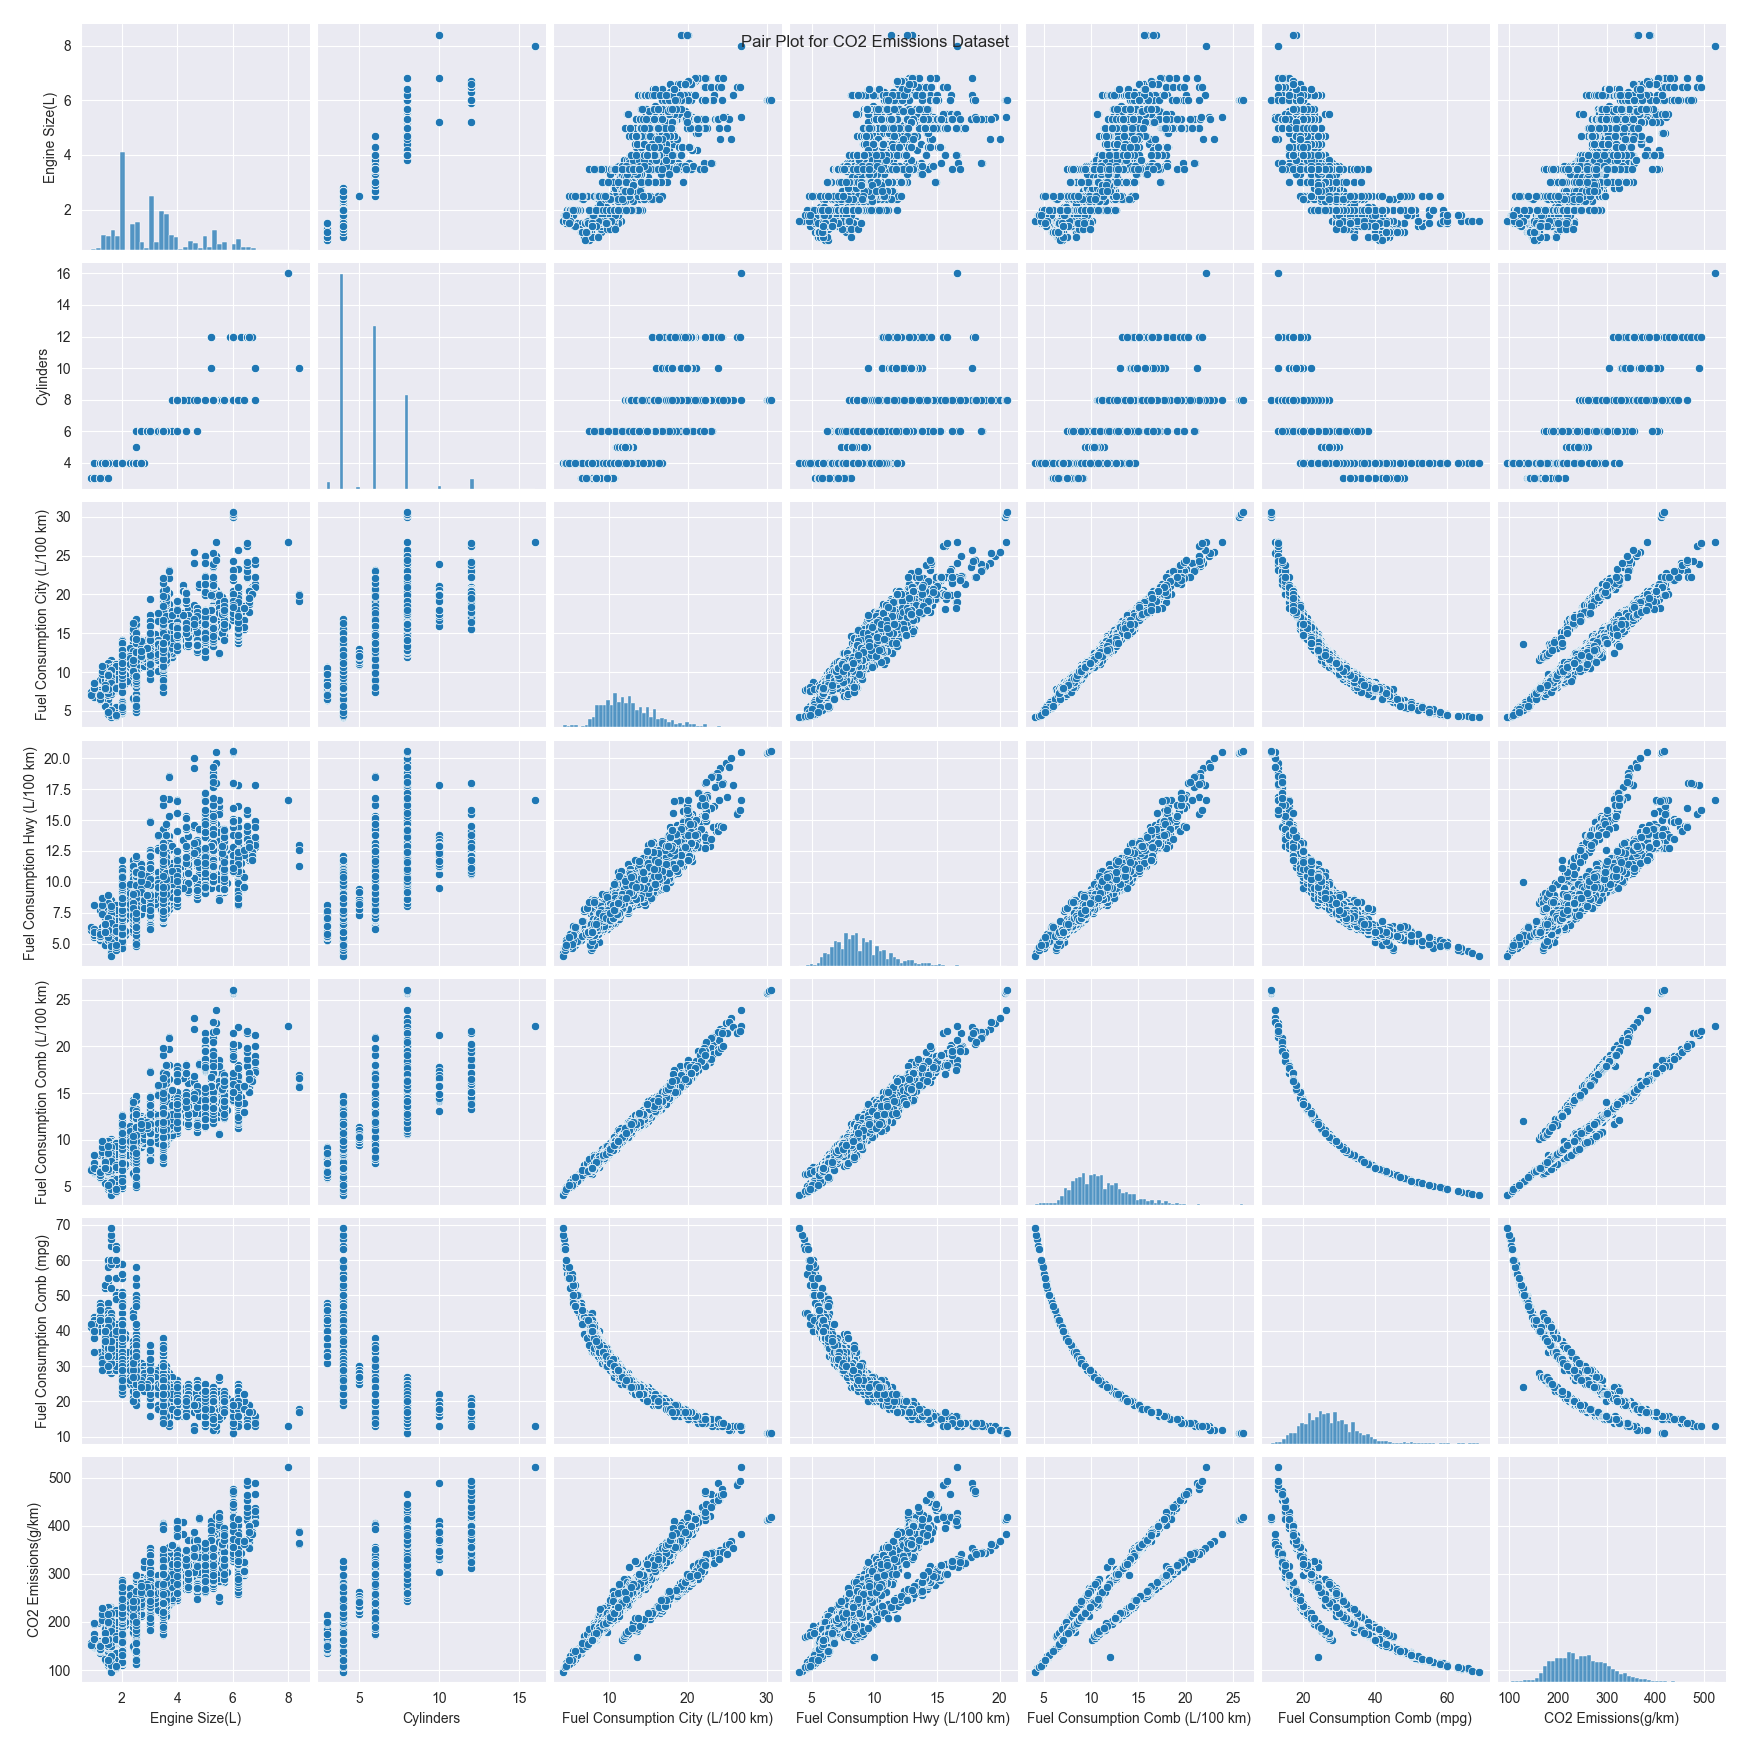
\includegraphics[width=0.95\textwidth]{./../Assets/pairplot.png}
        \caption{Pairplot of the features}
        \label{fig:pairplot}
    \end{figure}
    \vspace*{5pt} \\
    \begin{figure}[h]
        \centering
        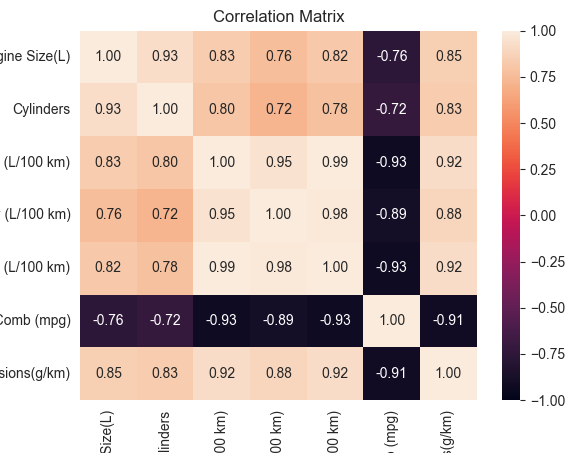
\includegraphics[width=0.6\textwidth]{./../Assets/correlation.png}
        \caption{Correlation matrix of the features}
        \label{fig:correlation}
    \end{figure}
    \begin{figure}[h]
        \centering
        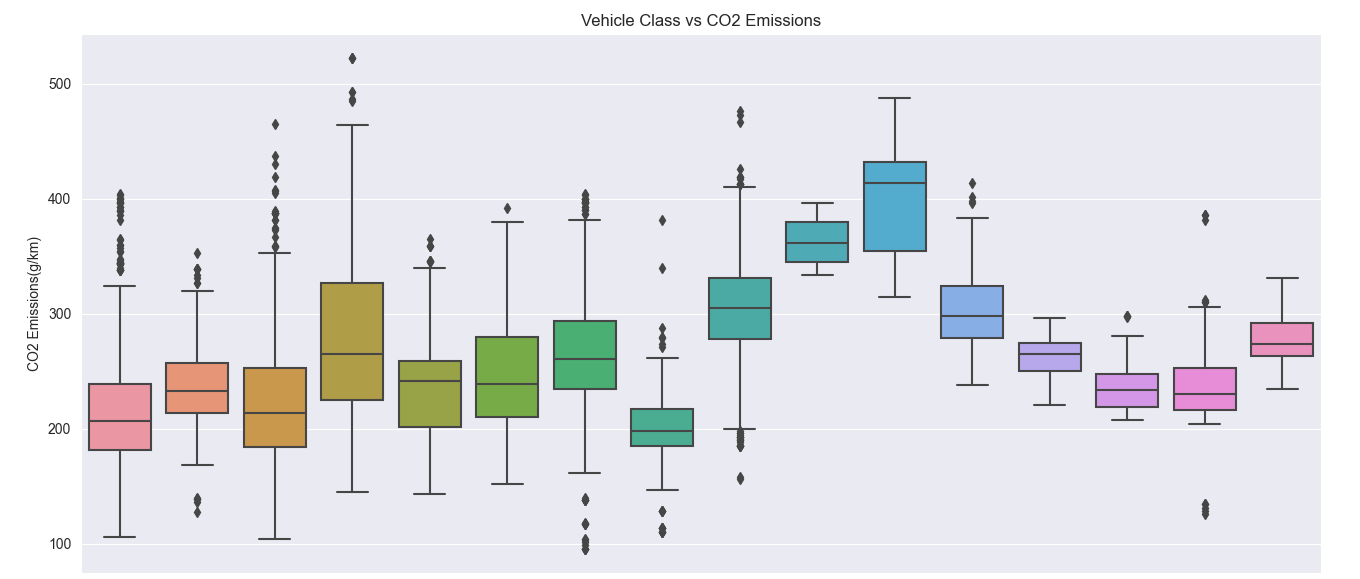
\includegraphics[width=0.6\textwidth]{./../Assets/box.png}
        \caption{Boxplot of \texttt{Vehicle Class} against \texttt{CO2 Emissions}}
        \label{fig:box}
    \end{figure}
    \vspace*{0pt} \\
    Figure \ref{fig:vehicle_class} shows the distribution of number of samples of each class of \texttt{Vehicle Class}.
    Clearly, the number of samples in each class is not balanced. This could lead to a bias in the model. However,
    since this is not the target variable, it is not a major concern.
    \begin{figure}[h]
        \centering
        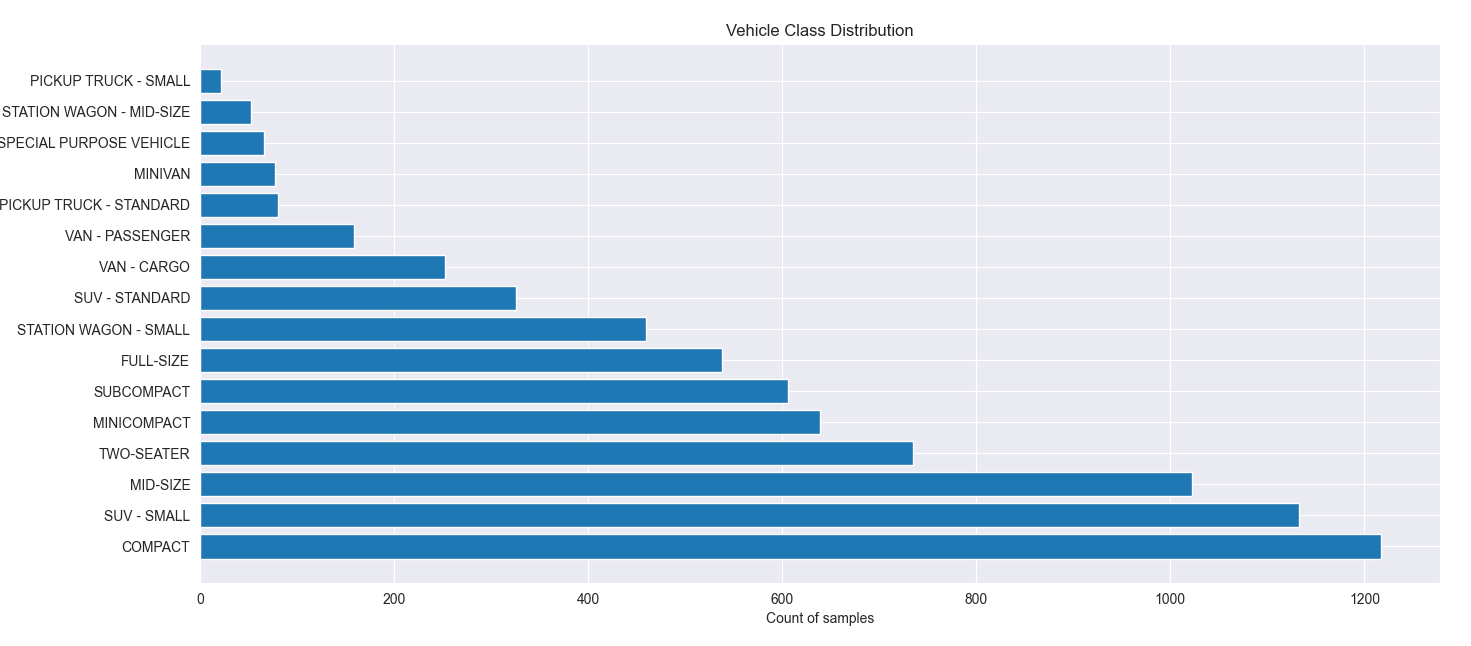
\includegraphics[width=0.85\textwidth]{./../Assets/vehicle_class.png}
        \caption{Distribution of number of samples of \texttt{Vehicle Class}}
        \label{fig:vehicle_class}
    \end{figure}

    \subsubsection*{Key Insights}
    With the above analysis, the important insights drawn from the data are summarized
    here.
    \begin{itemize}
        \item
        Most features show strong positive correlation with each other, apart from the feature \texttt{Fuel Consumption Comb (mpg)},
        which shows strong negative correlation with the all other features.
        \item
        \texttt{VAN - PASSENGER} has the highest average \texttt{CO2 Emissions (g/km)}, while the \texttt{Vehicle Class} of
        \texttt{STATION WAGON - SMALL} has the lowest, with a few outliers.
        \item
        The \texttt{Vehicle Class} of \texttt{COMPACT} has the highest number of samples, and \texttt{PICKUP TRUCK - SMALL}
        has the lowest number of samples in the dataset.
        \item
        The distribution of the target variable and \texttt{Fuel Consumption Comb (mpg)} are gaussian, with a slight skew to the left.
        \item
        The \texttt{Fuel Type} distribution suggests that the \texttt{Z} and \texttt{D} types dominate the dataset, while the
        \texttt{X} and \texttt{E} types are the least common.
        \item
        The pairplot suggests that the number of \texttt{Cylinders} in the engine shows high variation in correlating with the other features.
        \item
        The pairplot also displays that the \texttt{Engine Size} and \texttt{Fuel Consumption (L/100)} features are the most correlated with
        the target, \texttt{CO2 Emissions (g/km)}. The features with negative correlation are also evident.
        \item
        Overall, all features are strongly correlated with the target variable, which is a good indicator that the model will perform well.
    \end{itemize}

    \subsection*{Dataset Visualization using 2-dimensional $t$-SNE Algorithm}
    We use the $t$-Stochastic Neighbor Embedding Algorithm to reduce the dataset to 2 dimensions. This algorithm preserves the unnderlying
    structure of the dataset. So, ideally, the clusters in the data in higher dimensions should be preserved in the 2-dimensional visualization.
    \vspace*{5pt} \\
    The algorithm is applied on two separate copies of the dataset. One encodes categorical features using label encoding, and the other
    encodes categorical features using one-hot encoding. The numerical features are standardized before applying the algorithm.
    \vspace*{5pt} \\
    Figure \ref{fig:tsne} shows the 2-dimensional visualization of the dataset. It is clear from the visualization that the clusters are preserved.
    They are also well-separated. The data points are also not very sparsely or very densely distributed.
    In both plots, the data points are fairly separated, with very minute differences. This means that the model should perform
    well with both encodings.

    \begin{figure}[ht]
        \centering
        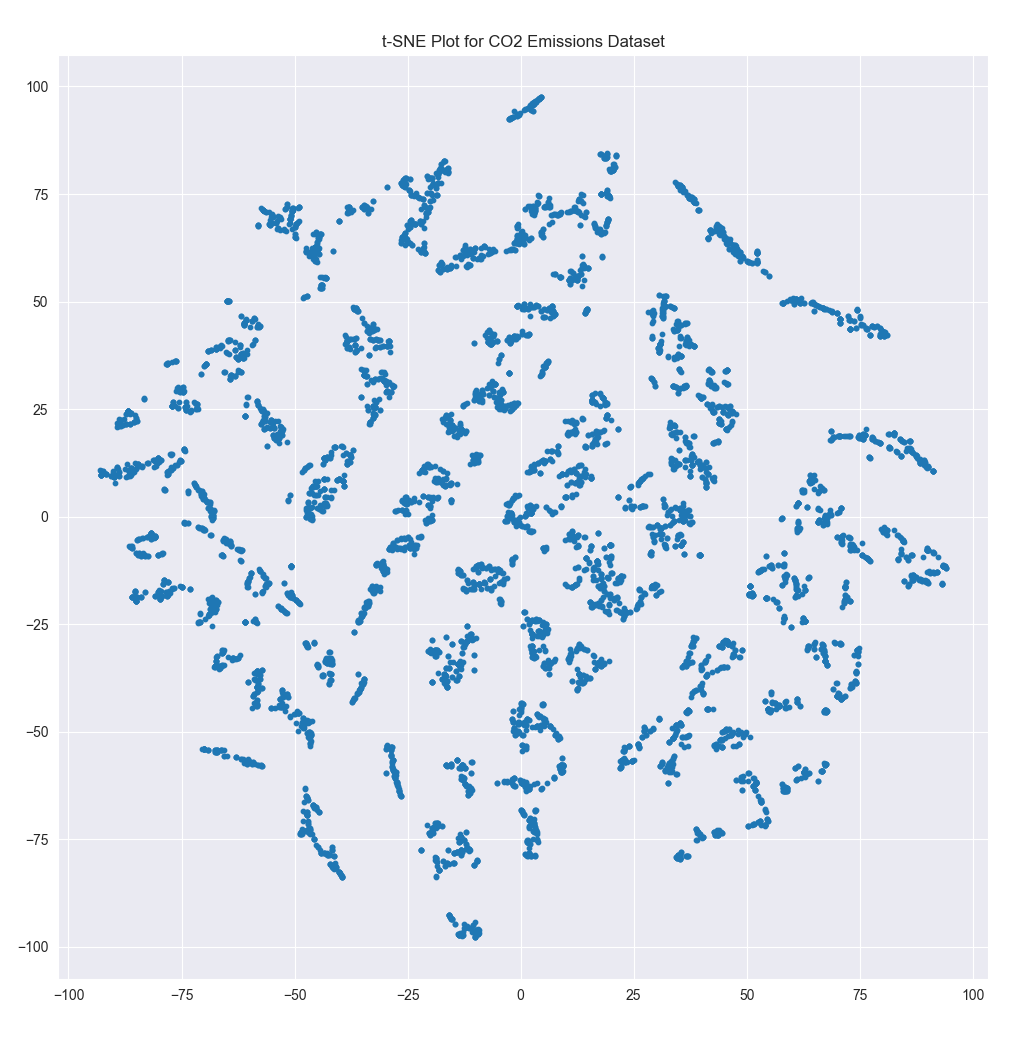
\includegraphics[width=0.45\textwidth]{./../Assets/tsne_1.png}
        \hfill
        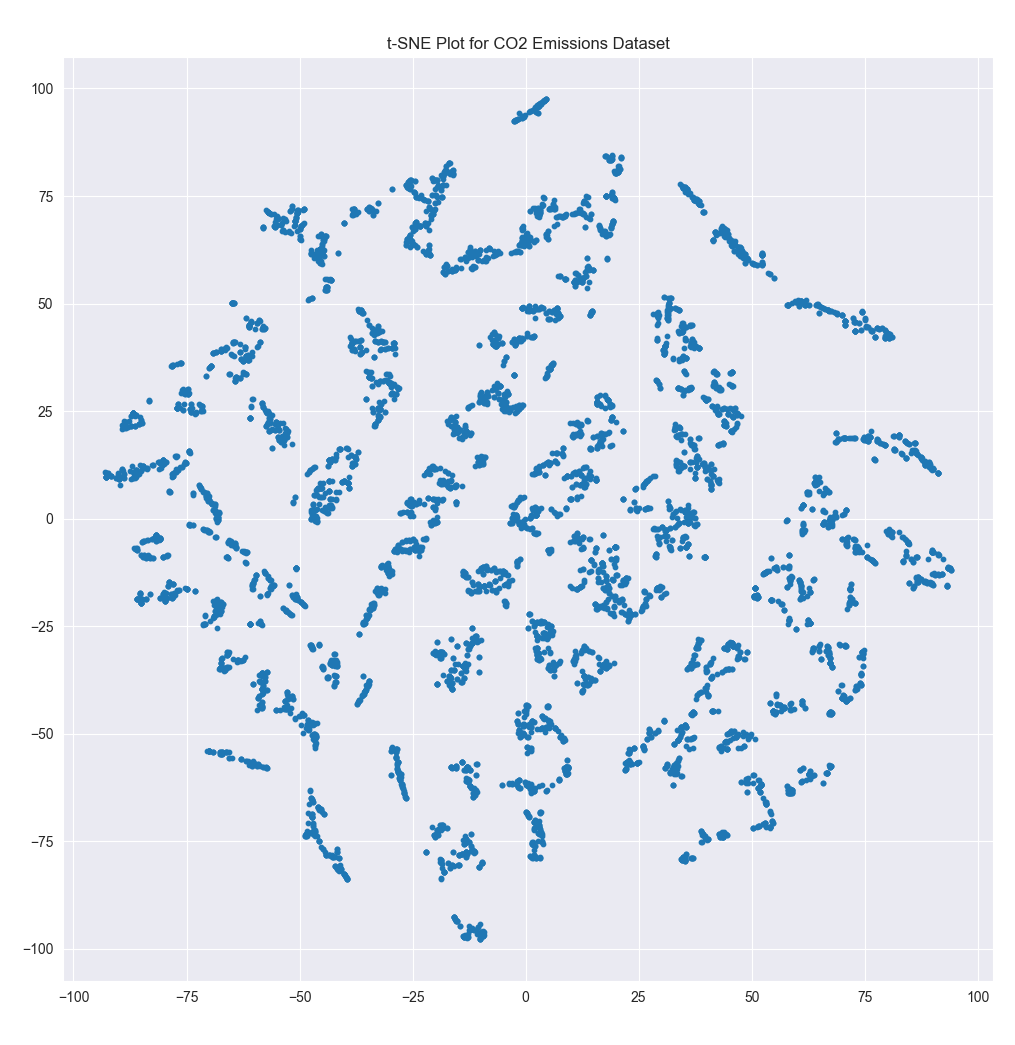
\includegraphics[width=0.45\textwidth]{./../Assets/tsne_2.png}
        \caption{2-dimensional $t$-SNE visualization of the dataset (Label and One-Hot Encoded)}
        \label{fig:tsne}
    \end{figure}

    \subsection*{Model Training}
    From this subsection, we use two variants of the dataset. The first has its categorical values encoded using Label Encoding,
    whereas we use One-Hot Encoding for the second variant. The numerical features are standardized to have zero mean and unit variance.
    The Label Encoder encodes the categorical features as integers, while the One-Hot Encoder encodes the categorical features as one-hot vectors.
    \vspace*{5pt} \\
    The tabulated results of all the different models trained are given in the following tables. The models were trained using
    different encodings, regressors, and hyperparameters. The MSE, RMSE, $R^{2}$-Score, Adjusted $R^{2}$-Score, and MAE are reported
    for each model.

    \subsubsection*{Linear Regression with Label Encoding}
    The results of the Linear Regression models trained with Label Encoded data are given in Table \ref{tab:linear_label}. A few models were also
    trained with PCA for different values of dimensions. This was done to check how the number of dimensions affects the performance of the model.
    \begin{table}[htbp]
        \centering
        \begin{tabular}{|c|l|c|c|c|c|c|}
            \hline
            \texttt{n} (PCA) & Dataset & MSE & RMSE & $R^{2}$-Score & Adj. $R^{2}$-Score & MAE \\
            \hline \hline
            - & \textsc{Train} & 283.0803 & 16.8249 & 0.9178 & 0.9177 & 10.9406 \\
            \hline
            - & \textsc{Test} & 306.8297 & 17.5165 & 0.9078 & 0.9071 & 11.3096 \\
            \hline
            4 & \textsc{Train} & 389.2899 & 19.7304 & 0.8858 & 0.8857 & 13.5305 \\
            \hline
            4 & \textsc{Test} & 441.0239 & 21.0006 & 0.8732 & 0.8728 & 14.7514 \\
            \hline
            6 & \textsc{Train} & 380.2578 & 19.5002 & 0.8885 & 0.8884 & 13.3269 \\
            \hline
            6 & \textsc{Test} & 436.2294 & 20.8861 & 0.8746 & 0.8740 & 14.5930 \\
            \hline
            8 & \textsc{Train} & 345.7971 & 18.5956 & 0.8986 & 0.8984 & 12.6924 \\
            \hline
            8 & \textsc{Test} & 394.8307 & 19.8703 & 0.8865 & 0.8858 & 13.9460 \\
            \hline
            10 & \textsc{Train} & 336.9742 & 18.3569 & 0.9012 & 0.9010 & 12.6153 \\
            \hline
            10 & \textsc{Test} & 383.4623 & 19.5822 & 0.8897 & 0.8890 & 13.8268 \\
            \hline
        \end{tabular}
        \caption{Results of different \texttt{LinearRegression} models trained using Label Encoding}
        \label{tab:linear_label}
    \end{table}

    \subsubsection*{Linear Regression with One-Hot Encoding}
    The results of the Linear Regression models trained with One-Hot Encoded data are given in Table \ref{tab:linear_onehot}. This is a
    repeat of the experiment done above, but for a different encoding of data. Surprisingly, almost all models trained with One-Hot Encoding
    perform significantly better than the models trained with Label Encoding.
    \vspace*{5pt} \\
    The model trained on the original dataset (One-Hot Encoded) performs the best, with an $R^{2}$-Score of $1.0$ and MSE of $3.01 \times 10^{-27}$
    on the testing data. This indicates that the model works almost perfectly. The models trained with PCA also perform well, but the performance
    is inversely proportional to the number of principal components selected.
    \begin{table}[htbp]
        \centering
        \begin{tabular}{|c|l|c|c|c|c|c|}
            \hline
            \texttt{n} (PCA) & Dataset & MSE & RMSE & $R^{2}$-Score & Adj. $R^{2}$-Score & MAE \\
            \hline \hline
            - & \textsc{Train} & 2.95 $\times 10^{-27}$ & 5.43 $\times 10^{-14} $ & 1.0 & 1.0 & 3.90 $\times 10^{-14}$ \\
            \hline
            - & \textsc{Test} & 3.01 $\times 10^{-27}$ & 5.49 $\times 10^{-14}$ & 1.0 & 1.0 & 3.92 $\times 10^{-14}$ \\
            \hline
            4 & \textsc{Train} & 387.6435 & 19.6887 & 0.8863 & 0.8862 & 13.5284 \\
            \hline
            4 & \textsc{Test} & 439.1840 & 20.9567 & 0.8737 & 0.8734 & 14.7233 \\
            \hline
            6 & \textsc{Train} & 364.7109 & 19.0974 & 0.8930 & 0.8929 & 13.0232 \\
            \hline
            6 & \textsc{Test} & 423.8275 & 20.5871 & 0.8781 & 0.8776 & 14.3517 \\
            \hline
            8 & \textsc{Train} & 340.8897 & 18.4632 & 0.9000 & 0.8999 & 12.7788 \\
            \hline
            8 & \textsc{Test} & 394.8174 & 19.8700 & 0.8865 & 0.8858 & 14.0380 \\
            \hline
            10 & \textsc{Train} & 325.2329 & 18.0342 & 0.9046 & 0.9045 & 12.2897 \\
            \hline
            10 & \textsc{Test} & 374.1246 & 19.3423 & 0.8924 & 0.8917 & 13.6176 \\
            \hline
        \end{tabular}
        \caption{Results of different \texttt{LinearRegression} models trained using One-Hot Encoding}
        \label{tab:linear_onehot}
    \end{table}

    \subsubsection*{Stochastic Gradient Descent Regression with different Encodings}
    We also implemented linear regression using the \texttt{SGDRegressor}, which uses Stochastic Gradient
    Descent to train the model. The results of the models trained with different encodings are given in Table \ref{tab:sgd}.
    \vspace*{5pt} \\
    Clearly, the one-hot encoded model outperforms the label encoded model. But both models perform well,
    and the performance is comparable with the usual \texttt{LinearRegression} model.
    \begin{table}[htbp]
        \centering
        \begin{tabular}{|l|l|c|c|c|c|c|}
            \hline
            Encoding & Dataset & MSE & RMSE & $R^{2}$-Score & Adj. $R^{2}$-Score & MAE \\
            \hline \hline
            \textsc{Label} & \textsc{Train} & 288.1083 & 16.9737 & 0.9164 & 0.9162 & 10.8516 \\
            \hline
            \textsc{Label} & \textsc{Test} & 314.9450 & 17.7466 & 0.9054 & 0.9046 & 11.2728 \\
            \hline
            \textsc{One-Hot} & \textsc{Train} & 0.0025 & 0.0501 & 0.9999 & 0.9999 & 0.0349 \\
            \hline
            \textsc{One-Hot} & \textsc{Test} & 0.0023 & 0.0486 & 0.9999 & 0.9999 & 0.0345 \\
            \hline
        \end{tabular}
        \caption{Results of different \texttt{SGDRegressor} models trained with different encodings}
        \label{tab:sgd}
    \end{table}

    \subsubsection*{Regression with Regularization}
    We subject the Linear Regression Models to $L_{1}$ (Lasso) and $L_{2}$ (Ridge) regularization.
    Ideally, regularization should reduce the variance in the model, and hence, avoid overfitting.
    \vspace*{5pt} \\
    Table \ref{tab:regularization} shows the results of the models trained with regularization.
    \begin{table}[htbp]
        \centering
        \begin{tabular}{|l|l|c|c|c|c|c|}
            \hline
            Regularization & Dataset & MSE & RMSE & $R^{2}$-Score & Adj. $R^{2}$-Score & MAE \\
            \hline \hline
            $L_{1}$ \textsc{(Lasso)} & \textsc{Train} & 1.00 $\times 10^{-4}$ & 0.0100 & 1.0 & 1.0 & 0.0079 \\
            \hline
            $L_{1}$ \textsc{(Lasso)} & \textsc{Test} & 9.81 $\times 10^{-5}$ & 0.0099 & 1.0 & 1.0 & 0.0078 \\
            \hline
            $L_{2}$ \textsc{(Ridge)} & \textsc{Train} & 1.15 $\times 10^{-7}$ & 0.0003 & 1.0 & 1.0 & 0.0002 \\
            \hline
            $L_{2}$ \textsc{(Ridge)} & \textsc{Test} & 1.09 $\times 10^{-7}$ & 0.0003 & 1.0 & 1.0 & 0.0002 \\
            \hline
        \end{tabular}
        \caption{Results of different regularization models on Linear Regression}
        \label{tab:regularization}
    \end{table}
    \vspace*{5pt} \\
    All the above models were trained with the regularization parameter $\lambda = 0.01$.
    Clearly, $L_{2}$ regularization works better than $L_{1}$ regularization. However, the $R^{2}$-Scores
    of both the models were equal to $1.0$. The MSE and MAE are also very low, but not as low as the regular
    one-hot encoded linear regression models, which is ideal.

    \vfill

    \section*{References}
    \begin{enumerate}
        \item \href{https://en.wikipedia.org/wiki/Logistic_function}{\color{blue}\underline{Wikipedia: Logistic Function}}
        \item \href{https://www.tutorialspoint.com/how-to-find-residual-variance-of-a-linear-regression-model-in-r}{\color{blue}\underline{Estimating variance in Linear Regression in $\mathbb{R}$}}
        \item \href{https://www.geeksforgeeks.org/confusion-matrix-machine-learning/}{\color{blue}\underline{Confusion Matrix, Accuracy, Precision, Recall, F1-Score - GeeksForGeeks}}
        \item \href{https://www.geeksforgeeks.org/regularization-in-machine-learning/}{\color{blue}\underline{Regularization - GeeksForGeeks Guide}}
        \item \href{https://byjus.com/maths/box-plot/}{\color{blue}\underline{Box Plot - Byjus}}
        \item \href{https://scikit-learn.org/stable/modules/generated/sklearn.manifold.TSNE.html}{\color{blue}\underline{$t$-SNE Manifold - \texttt{scikit-learn} official documentation}}
    \end{enumerate}

\end{document}